\pagestyle{mystyle}
\chapter{Analisi dei Requisiti e Progettazione del Sistema}
\label{chap:requirements_design}
\label{chap:progettazione}

Il capitolo traduce il quadro teorico introdotto in precedenza in un problema
progettuale concreto. L'obiettivo non è costruire un sistema RAG generico, ma
integrare un assistente nel contesto operativo di Intré, rispettando i vincoli
organizzativi, infrastrutturali e di riservatezza già presenti. L'analisi
parte quindi dal modello aziendale delle Gilde, identifica il caso d'uso e
il corpus disponibile, formalizza i requisiti e motiva le
scelte tecnologiche che portano alla proposta architetturale.

% -------------------------------------------------------------
\section{Il contesto aziendale: Intré S.r.l.}
\label{sec:intre_context}
% -------------------------------------------------------------
Intré S.r.l.\footnote{\url{https://www.intre.it}} è una software factory
italiana con sede a Monza che sviluppa prodotti digitali per settori eterogenei,
tra cui energia, assicurazioni, automotive ed entertainment, organizzando il
lavoro in team Scrum cross-funzionali. La dimensione aziendale, pari a circa
settanta persone, consente di mantenere processi interni formalizzati senza
rinunciare a una circolazione diretta della conoscenza tra i
team~\cite{intre_learning_organization}.

Il payoff \emph{Learn / Code / Deploy Value} esplicita l'ordine con cui Intré
interpreta il proprio modo di produrre valore: prima l'apprendimento, poi la
realizzazione del software, infine il rilascio di valore al cliente. Questa
impostazione è coerente con il concetto di \textit{Learning Organization}
proposto da Peter Senge in \emph{The Fifth Discipline}~\cite{senge1990fifth}.
Nel modello di Senge l'apprendimento organizzativo non coincide con la sola
formazione individuale, ma richiede padronanza personale, modelli mentali
esplicitati, visione condivisa, apprendimento di gruppo e pensiero sistemico.
La quinta disciplina, cioè il pensiero sistemico, collega le altre quattro e
permette di leggere l'organizzazione come un insieme di relazioni, feedback e
dipendenze, non come una somma di attività isolate.

Nel caso di Intré questa prospettiva non rimane un principio astratto. Il
modello aziendale prevede un insieme di pratiche dedicate all'apprendimento
continuo: Gilde, Camp, Community, Skill Matrix, certificazioni, Academy,
Community of Practice per speaker, obiettivi di apprendimento, formazione in
aula e corsi di lingua~\cite{intre_learning_organization}. Tali pratiche
rendono l'apprendimento una responsabilità distribuita, sostenuta da tempo,
budget e momenti di restituzione pubblica. La certificazione ISO~27001 e le
competenze maturate in ambiti come cloud-native, cybersecurity e intelligenza
artificiale rendono inoltre particolarmente rilevante il tema della gestione
sicura della conoscenza interna.

\subsection{Il modello delle Gilde}
\label{subsec:guild_model}
Le \textbf{Gilde} (\emph{gilde}) sono uno degli strumenti principali con cui
Intré rende operativa la propria idea di apprendimento organizzativo. Sono cicli
rapidi di apprendimento di gruppo, della durata di quattro mesi, costruiti a
partire da temi proposti direttamente dalle persone
dell'azienda~\cite{intre_learning_organization,intre_gilde}. Una Gilda nasce quando una
proposta raccoglie un numero minimo di partecipanti; il gruppo lavora in
autogestione e dedica al tema scelto una quota stabile del proprio tempo
lavorativo. L'esito non è un esame o una valutazione formale, ma un risultato
di apprendimento da presentare al Camp successivo. Il modello combina quindi
autonomia nella scelta dei temi, durata definita, lavoro di gruppo e produzione
di un risultato condivisibile. Le sue caratteristiche principali sono:

\begin{itemize}
  \item \textbf{Formazione spontanea}: ogni persona può proporre o aderire a
    una Gilda su qualsiasi argomento, tecnico o non tecnico (es. linguaggi
    di programmazione, ceramica, game development, intelligenza artificiale).
  \item \textbf{Ciclo temporale (Epoch)}: le Gilde si ricreano ogni quattro
    mesi; ogni ciclo costituisce un'``epoca'' distinta, con nuovi temi e nuovi
    gruppi. Questa scansione periodica evita che l'apprendimento rimanga legato
    a iniziative isolate e lo inserisce in una routine aziendale riconoscibile.
  \item \textbf{Output condivisibile}: al termine del periodo la Gilda produce
    un risultato tangibile (prototipo, report, repository, presentazione) che
    viene archiviato e condiviso. La restituzione pubblica durante il Camp
    trasforma l'esperienza del gruppo in conoscenza disponibile anche per il
    resto dell'organizzazione.
  \item \textbf{Ampiezza tematica}: dall'archivio pubblico del sito aziendale
    emergono Gilde su temi come \emph{Angular}, \emph{F\#}, \emph{IA agentiva},
    \emph{game development} con Phaser, ceramica, selezione fotografica con AI,
    e molti altri~\cite{intre_gilde}.
\end{itemize}

Il ciclo di vita delle Gilde è gestito tramite \textbf{i3Guild}, una
piattaforma web interna sviluppata con Next.js, PostgreSQL e Keycloak. Questa
applicazione conserva nel tempo proposte, descrizioni, partecipanti e risultati
delle Gilde. Di conseguenza, i3Guild non è soltanto uno strumento
amministrativo: è una memoria organizzativa parziale, nella quale si depositano
interessi, competenze, esperimenti e risultati prodotti nel tempo. Proprio per
questo rappresenta sia il contesto applicativo di integrazione sia la
principale sorgente dati del sistema RAG progettato in questa tesi.

% -------------------------------------------------------------
\section{Caso d'uso: Proposta di nuove Gilde}
\label{sec:use_case_intre}
% -------------------------------------------------------------

Il caso d'uso individuato riguarda il supporto alla proposta di nuove Gilde.
Quando una persona vuole avviare una nuova iniziativa, può essere utile
conoscere esperienze precedenti, temi già affrontati, risultati ottenuti e
partecipanti coinvolti. Oggi queste informazioni esistono, ma sono distribuite
tra database e contenuti editoriali. Il sistema proposto mira a renderle
consultabili tramite query in linguaggio naturale, generando risposte
contestualizzate e ancorate a fonti interne. A tale scopo viene adottato il
paradigma \emph{Retrieval-Augmented Generation} (RAG), introdotto da Lewis et
al.~\cite{lewis2020retrieval} per estendere la memoria non parametrica dei Large
Language Model (LLM) tramite recupero dinamico di documenti da un corpus
esterno.

\subsection{Motivazione del caso d'uso}

Il corpus delle Gilde archiviate in i3Guild, insieme ai relativi blog post,
costituisce una base di conoscenza aziendale di valore: raccoglie descrizioni di
progetti, obiettivi, rischi, risultati raggiunti e annotazioni dei partecipanti,
accumulate in oltre trenta epoch a partire dal 2016~\cite{intre_gilde}. Tuttavia
questa conoscenza è frammentata. Una parte risiede in un database relazionale,
ottimo come sorgente applicativa ma poco accessibile tramite domande in
linguaggio naturale; un'altra parte è distribuita in post e contenuti non
sempre facili da reperire. Un assistente RAG consente di trasformare tale
patrimonio in uno strumento operativo: riduce il tempo di ricerca, facilita il
riuso delle esperienze pregresse e rende più trasferibile la conoscenza tra i
team.

\subsection{Obiettivi del caso d'uso}

Gli obiettivi del caso d'uso derivano direttamente dalla natura del corpus e dal
contesto aziendale in cui il sistema deve essere inserito. Il sistema deve
fornire risposte affidabili e tracciabili sui contenuti presenti nei repository
aziendali, riducendo il rischio di allucinazioni tipico della generazione
puramente parametrica~\cite{lewis2020retrieval}, e deve rendere più rapido il recupero
di informazioni utili per attività operative e decisionali interne a Intré.
Questi obiettivi devono essere raggiunti senza spostare i dati fuori
dall'infrastruttura aziendale, in coerenza con i requisiti di sovranità del dato
e con il Regolamento Generale sulla Protezione dei Dati
(GDPR)~\cite{gdpr2016}. L'integrazione, inoltre, deve inserirsi nel flusso
i3Guild esistente senza alterare il processo operativo già consolidato.

\subsection{Descrizione dei dati e analisi del corpus}
\label{subsec:data_analysis}

Per progettare correttamente la pipeline di ingestione è necessario chiarire
quali informazioni debbano alimentare l'indice. I dati di ingresso al sistema
RAG comprendono tre categorie:

\begin{itemize}
  \item \textbf{Documenti delle Gilde}: specifiche di progetto, obiettivi,
    rischi, risultati attesi e raggiunti, annotati con metadati strutturati
    (epoche, partecipanti, modalità di partecipazione).
  \item \textbf{Blog post}: post pubblicati dai partecipanti alle gilde che ne 
    sintetizzano i risultati e le esperienze maturate.
  \item \textbf{Documenti non strutturati}: file PDF, HTML e note operative con
    metadati associati.
\end{itemize}

Dall'analisi del corpus i3Guild, estratto il 15/02/2026, emergono le
statistiche riportate nelle Tabelle~\ref{tab:entity_stats}
e~\ref{tab:field_stats}. Questi valori non hanno solo funzione descrittiva:
determinano la granularità dell'indicizzazione, la strategia di chunking e la
scelta del modello di embedding.

\begin{table}[ht]
  \centering
  \caption{Statistiche delle entità principali del corpus i3Guild
    (estrazione 15/02/2026).}
  \label{tab:entity_stats}
  \small
  \begin{tabular}{lrp{7cm}}
    \toprule
    \textbf{Entità} & \textbf{Conteggio} & \textbf{Note} \\
    \midrule
    Gilda & 270 & Gestibile per re-indicizzazioni complete \\
    Epoch & 30 & $\approx$ 9 gilde per epoca in media \\
    Relazioni Utente-Gilda & 1.166 & $\approx$ 4,3 partecipanti medi per gilda \\
    Utenti esterni & 3 & Trascurabile ai fini del RAG \\
    \bottomrule
  \end{tabular}
\end{table}

\begin{table}[ht]
  \centering
  \caption{Statistiche dei campi testuali delle entità Gilda (valori in
    caratteri).}
  \label{tab:field_stats}
  \small
  \begin{tabular}{lrrrrl}
    \toprule
    \textbf{Campo} & \textbf{Media} & \textbf{Min} & \textbf{Max} &
      \textbf{Vuoti} & \textbf{Note} \\
    \midrule
    \texttt{summary} & 610 & 0 & 18.224 & 5\% & Campo più ricco; outlier
      rilevante \\
    \texttt{goals} & 258 & 0 & 2.698 & 35\% & Spesso breve o assente \\
    \texttt{outcome} & 133 & 0 & 2.145 & 36\% & Spesso breve o assente \\
    \texttt{risks} & 106 & 0 & 1.245 & 38\% & Spesso breve o assente \\
    \texttt{achievedResultsDescription} & 782 & 0 & 6.421 & 74\% & Lungo quando
      presente \\
    \texttt{journal} & $\approx$1 & 1 & 1 & 99\% & Praticamente inutilizzato;
      escluso \\
    \bottomrule
  \end{tabular}
\end{table}

\noindent La somma media dei campi testuali rilevanti della Gilda, inclusi
sommario, obiettivi, rischi, outcome e risultati raggiunti, ammonta a circa
1.900~caratteri,
corrispondenti a circa 400~token. Anche nel caso peggiore la somma non supera
i 7.000--8.000~token, rimanendo compatibile con la finestra di contesto del
modello di embedding selezionato (Sezione~\ref{subsec:embedding_choice}).
Da ciò deriva una conseguenza progettuale importante: nella maggior parte dei
casi una Gilda può essere trattata come documento consolidato, senza frammentare
aggressivamente i campi testuali e senza perdere il contesto semantico che lega
obiettivi, rischi e risultati.

\subsection{Struttura informativa delle Gilde e implicazioni per il retrieval}
\label{subsec:guild_information_structure}

L'analisi dello schema dati i3Guild conferma che la Gilda è l'unità informativa
più adatta all'indicizzazione. La tabella \texttt{Guild} raccoglie campi
descrittivi, campi progettuali e metadati organizzativi: nome, sommario,
obiettivi, opportunità, risultati attesi, rischi, risorse, budget, modalità di
partecipazione, riferimento all'epoch e descrizione dei risultati raggiunti. Le
tabelle collegate hanno un ruolo diverso. \texttt{Epoch} fornisce il contesto
temporale; \texttt{GuildUserRelation} collega partecipanti, Gilde ed epoch;
\texttt{GuildAchievedResult} contiene allegati binari, dei quali in questa fase
può essere indicizzato solo il nome del file, salvo introdurre una pipeline
dedicata di estrazione testuale.

Questa distinzione separa contenuto da metadato. I campi testuali della Gilda
alimentano embedding e ricerca semantica; epoch, partecipanti, modalità di
partecipazione e identificativi restano nel payload strutturato e servono per
filtrare o contestualizzare la risposta. La separazione evita due problemi:
inserire nel testo indicizzato informazioni poco semantiche, come identificativi
o date, e perdere però la possibilità di rispondere a domande operative che
richiedono vincoli strutturati. Una domanda come ``quali Gilde sull'intelligenza
artificiale sono state proposte in una certa epoch?'' richiede entrambe le
componenti: similarità semantica sul tema e filtro temporale sull'epoch.
La Tabella~\ref{tab:guild_retrieval_roles} riassume questa separazione tra
campi testuali, metadati e uso effettivo nella pipeline.

\begin{table}[ht]
  \centering
  \caption{Ruolo dei principali dati i3Guild nella pipeline RAG}
  \label{tab:guild_retrieval_roles}
  \small
  \begin{tabular}{L{3.2cm}L{4.8cm}L{5.3cm}}
    \toprule
    \textbf{Elemento} & \textbf{Informazione disponibile} &
      \textbf{Uso nella pipeline} \\
    \midrule
    \texttt{Guild} & Nome, sommario, obiettivi, opportunità, outcome, rischi,
      risorse, budget, risultati raggiunti &
      Documento principale da incorporare e recuperare semanticamente. \\
    \texttt{Epoch} & Inizio e fine del ciclo di Gilde &
      Filtro temporale e contesto della risposta. \\
    \texttt{GuildUserRelation} & Partecipante, Gilda, epoch, data di adesione &
      Payload per domande su partecipazione e composizione dei gruppi. \\
    \texttt{GuildAchievedResult} & File allegati e nome del file &
      Fonte secondaria; il contenuto binario richiede estrazione separata. \\
    \texttt{GuildDraft} & Proposte non ancora consolidate &
      Esclusa dall'indice principale se non validata come conoscenza storica. \\
    \bottomrule
  \end{tabular}
\end{table}

Gli esempi presenti nella documentazione interna del progetto chiariscono il
tipo di interrogazioni attese. Una query esplorativa come ``vorrei fondare una
gilda sulla musicà' deve essere ridotta ai termini informativi principali e
recuperare Gilde tematicamente vicine, ad esempio \emph{The Rolling Updates} o
\emph{Visual note for piano}, quando presenti nel corpus indicizzato. Domande
come ``quali Gilde si occupano di AI?'' privilegiano invece il recupero
semantico su \texttt{summary}, \texttt{goals} e \texttt{achievedResultsDescription};
domande come ``chi ha partecipato alla Gilda X?'' o ``quali erano i rischi
della Gilda Y?'' richiedono il raccordo tra retrieval, metadati e campi
specifici. Il corpus, quindi, non è una semplice collezione di testi: è un
insieme di documenti con struttura interna, relazioni e vincoli temporali.

Da questa analisi deriva la scelta di costruire documenti consolidati con
etichette di campo esplicite, ad esempio \texttt{[SOMMARIO]},
\texttt{[OBIETTIVI]}, \texttt{[RISCHI]} e
\texttt{[RISULTATI RAGGIUNTI]}. Le etichette mantengono riconoscibile la
provenienza dell'informazione anche dopo la concatenazione dei campi e aiutano
il generatore a distinguere tra intenzioni, rischi e risultati effettivamente
raggiunti. La strategia è coerente con le dimensioni osservate: poiché la Gilda
media rimane breve, il documento consolidato conserva più contesto rispetto a
una segmentazione per singolo campo, senza introdurre un carico eccessivo per
il modello di embedding.

% Segnaposto figura caso d'uso
La Figura~\ref{fig:intre_usecase} colloca il caso d'uso nel perimetro
applicativo, distinguendo attore, sistema i3Guild e componente RAG.

\begin{figure}[ht]
  \centering
  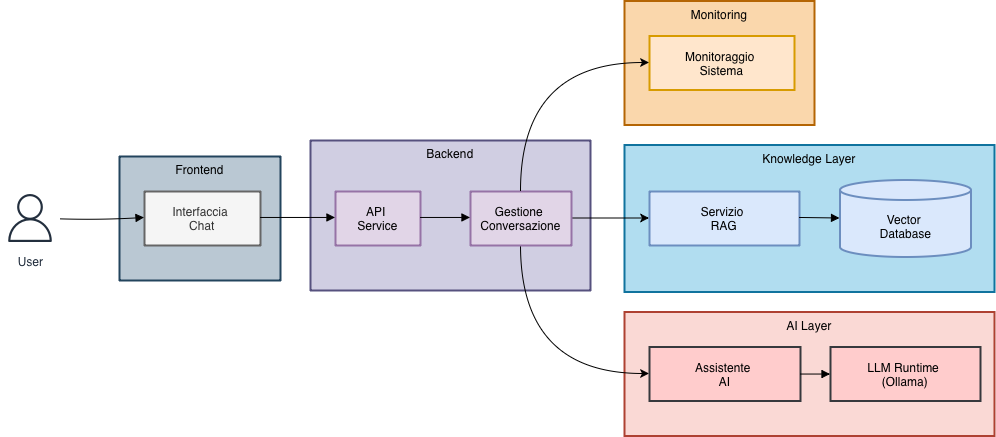
\includegraphics[width=0.75\textwidth]{chapter2/images/intre_usecase.png}
  \caption{Diagramma del caso d'uso ``Intré'': attori, interazioni principali e
    confini del sistema.}
  \label{fig:intre_usecase}
\end{figure}

\subsection{Scenario applicativo}
\label{subsec:application_scenario}

Lo scenario operativo previsto per il prototipo si colloca nel flusso già
presente in i3Guild. La Figura~\ref{fig:i3guild_guilds_list_screenshot} mostra
la consultazione dell'archivio delle Gilde, mentre la
Figura~\ref{fig:i3guild_guild_detail_screenshot} riporta il dettaglio di una
singola Gilda. La Figura~\ref{fig:i3guild_rag_screenshot} mostra invece il
punto in cui l'utente interroga l'assistente RAG in linguaggio naturale. La
sequenza rende visibile sia la sorgente applicativa da cui viene costruito il
corpus sia il punto in cui il prototipo espone il retrieval all'interno
dell'interfaccia.

\begin{figure}[ht]
  \centering
  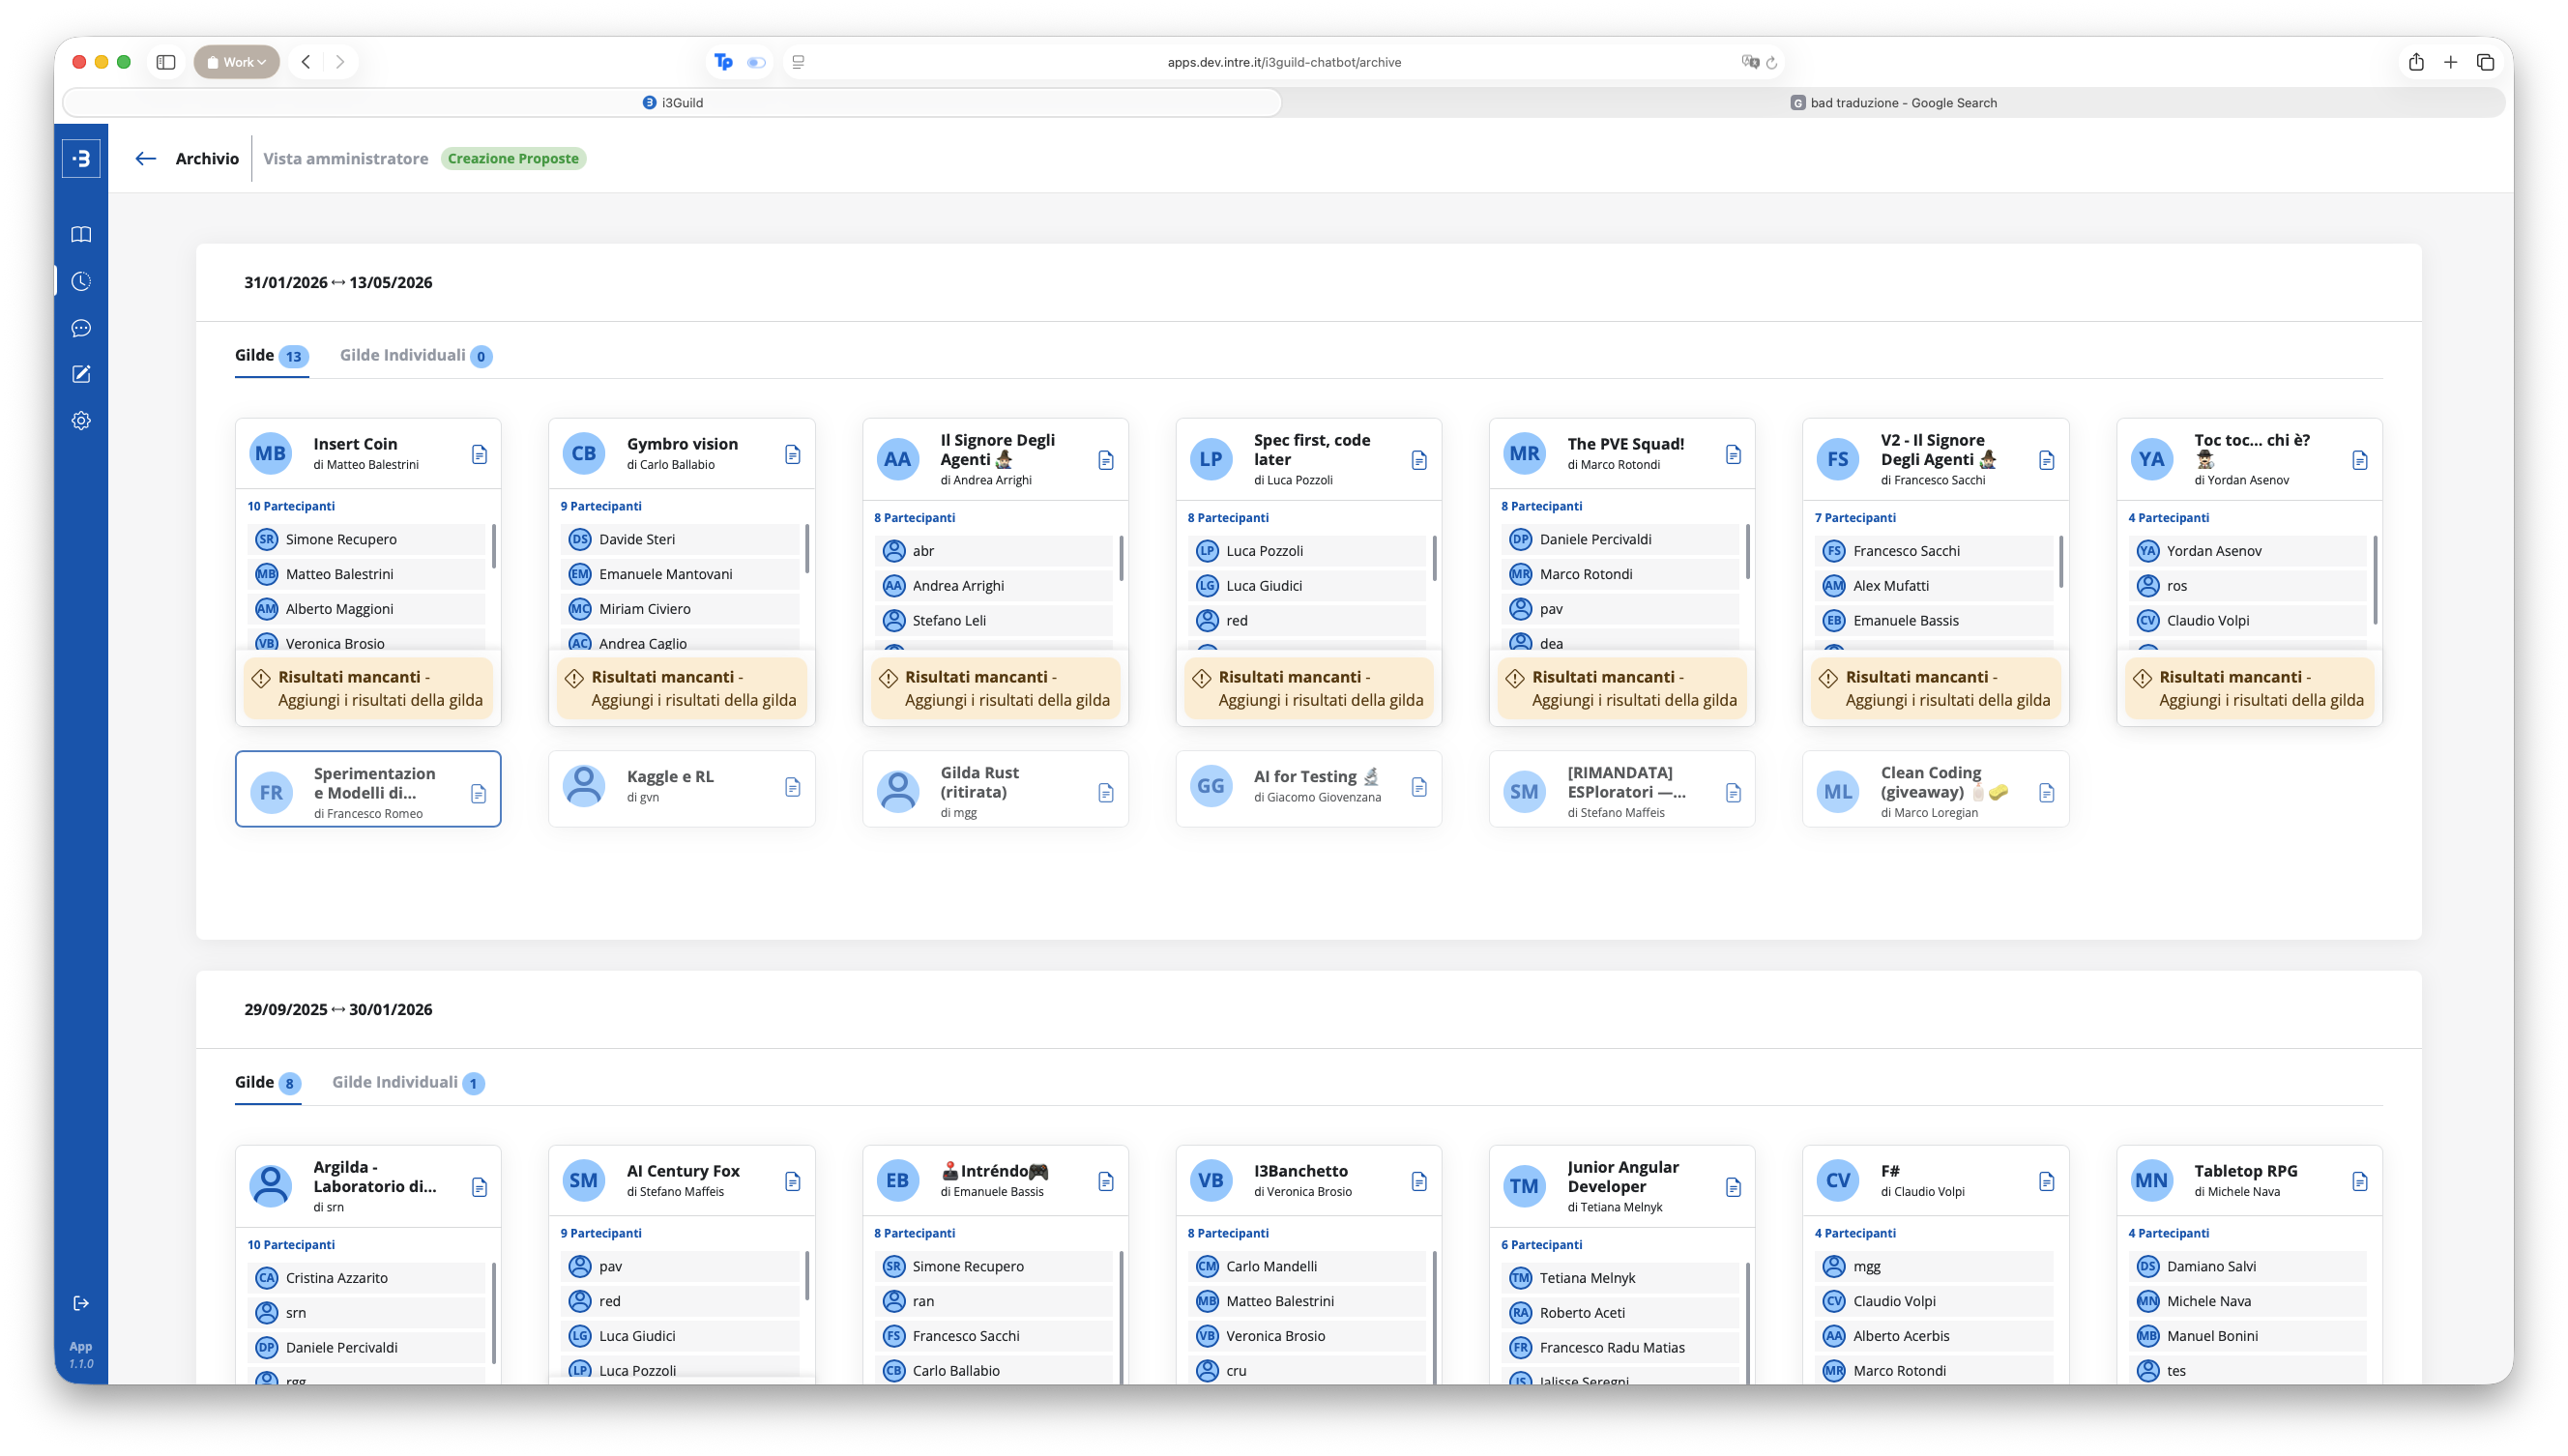
\includegraphics[width=0.95\textwidth]{chapter2/images/gilde.png}
  \caption{Vista dell'archivio delle Gilde nell'interfaccia i3Guild. La
    schermata mostra il punto di accesso al corpus applicativo usato dal
    sistema RAG.}
  \label{fig:i3guild_guilds_list_screenshot}
\end{figure}

\begin{figure}[ht]
  \centering
  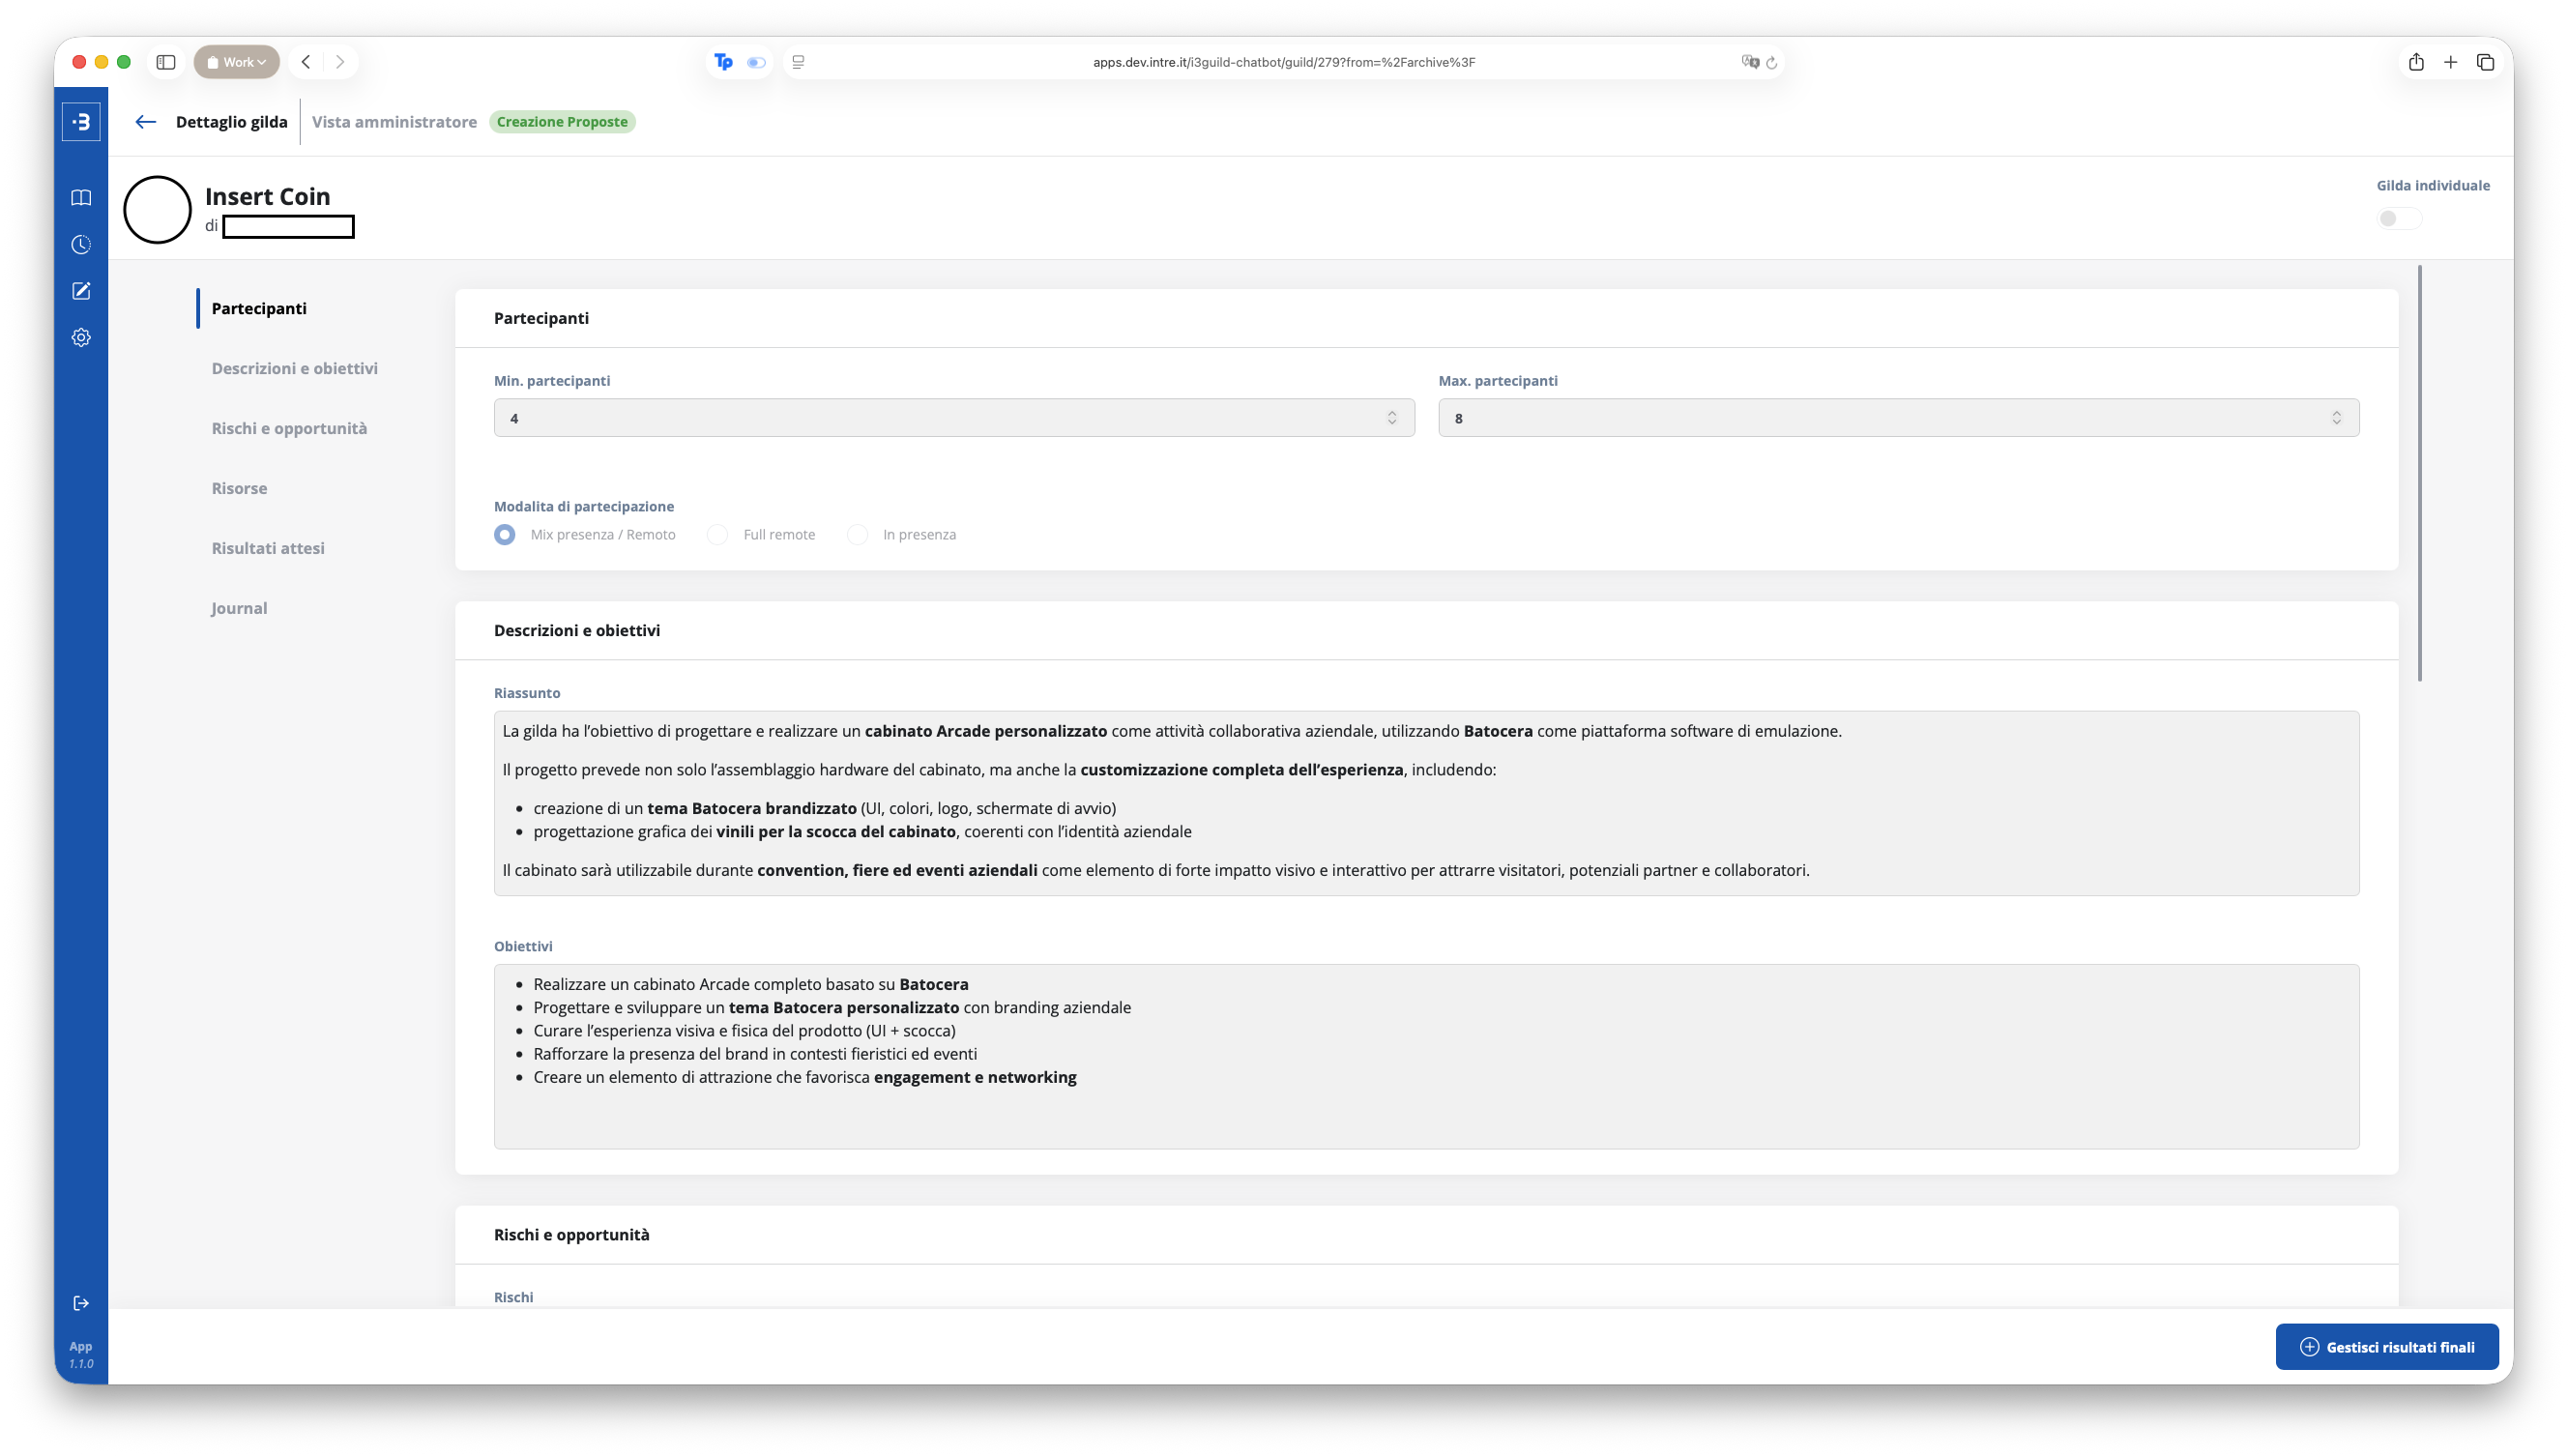
\includegraphics[width=0.95\textwidth]{chapter2/images/esempio_gilda.png}
  \caption{Dettaglio di una Gilda in i3Guild. I campi descrittivi e i metadati
    visualizzati nella pagina costituiscono parte delle informazioni trasformate
    in documenti indicizzabili.}
  \label{fig:i3guild_guild_detail_screenshot}
\end{figure}

\begin{figure}[ht]
  \centering
  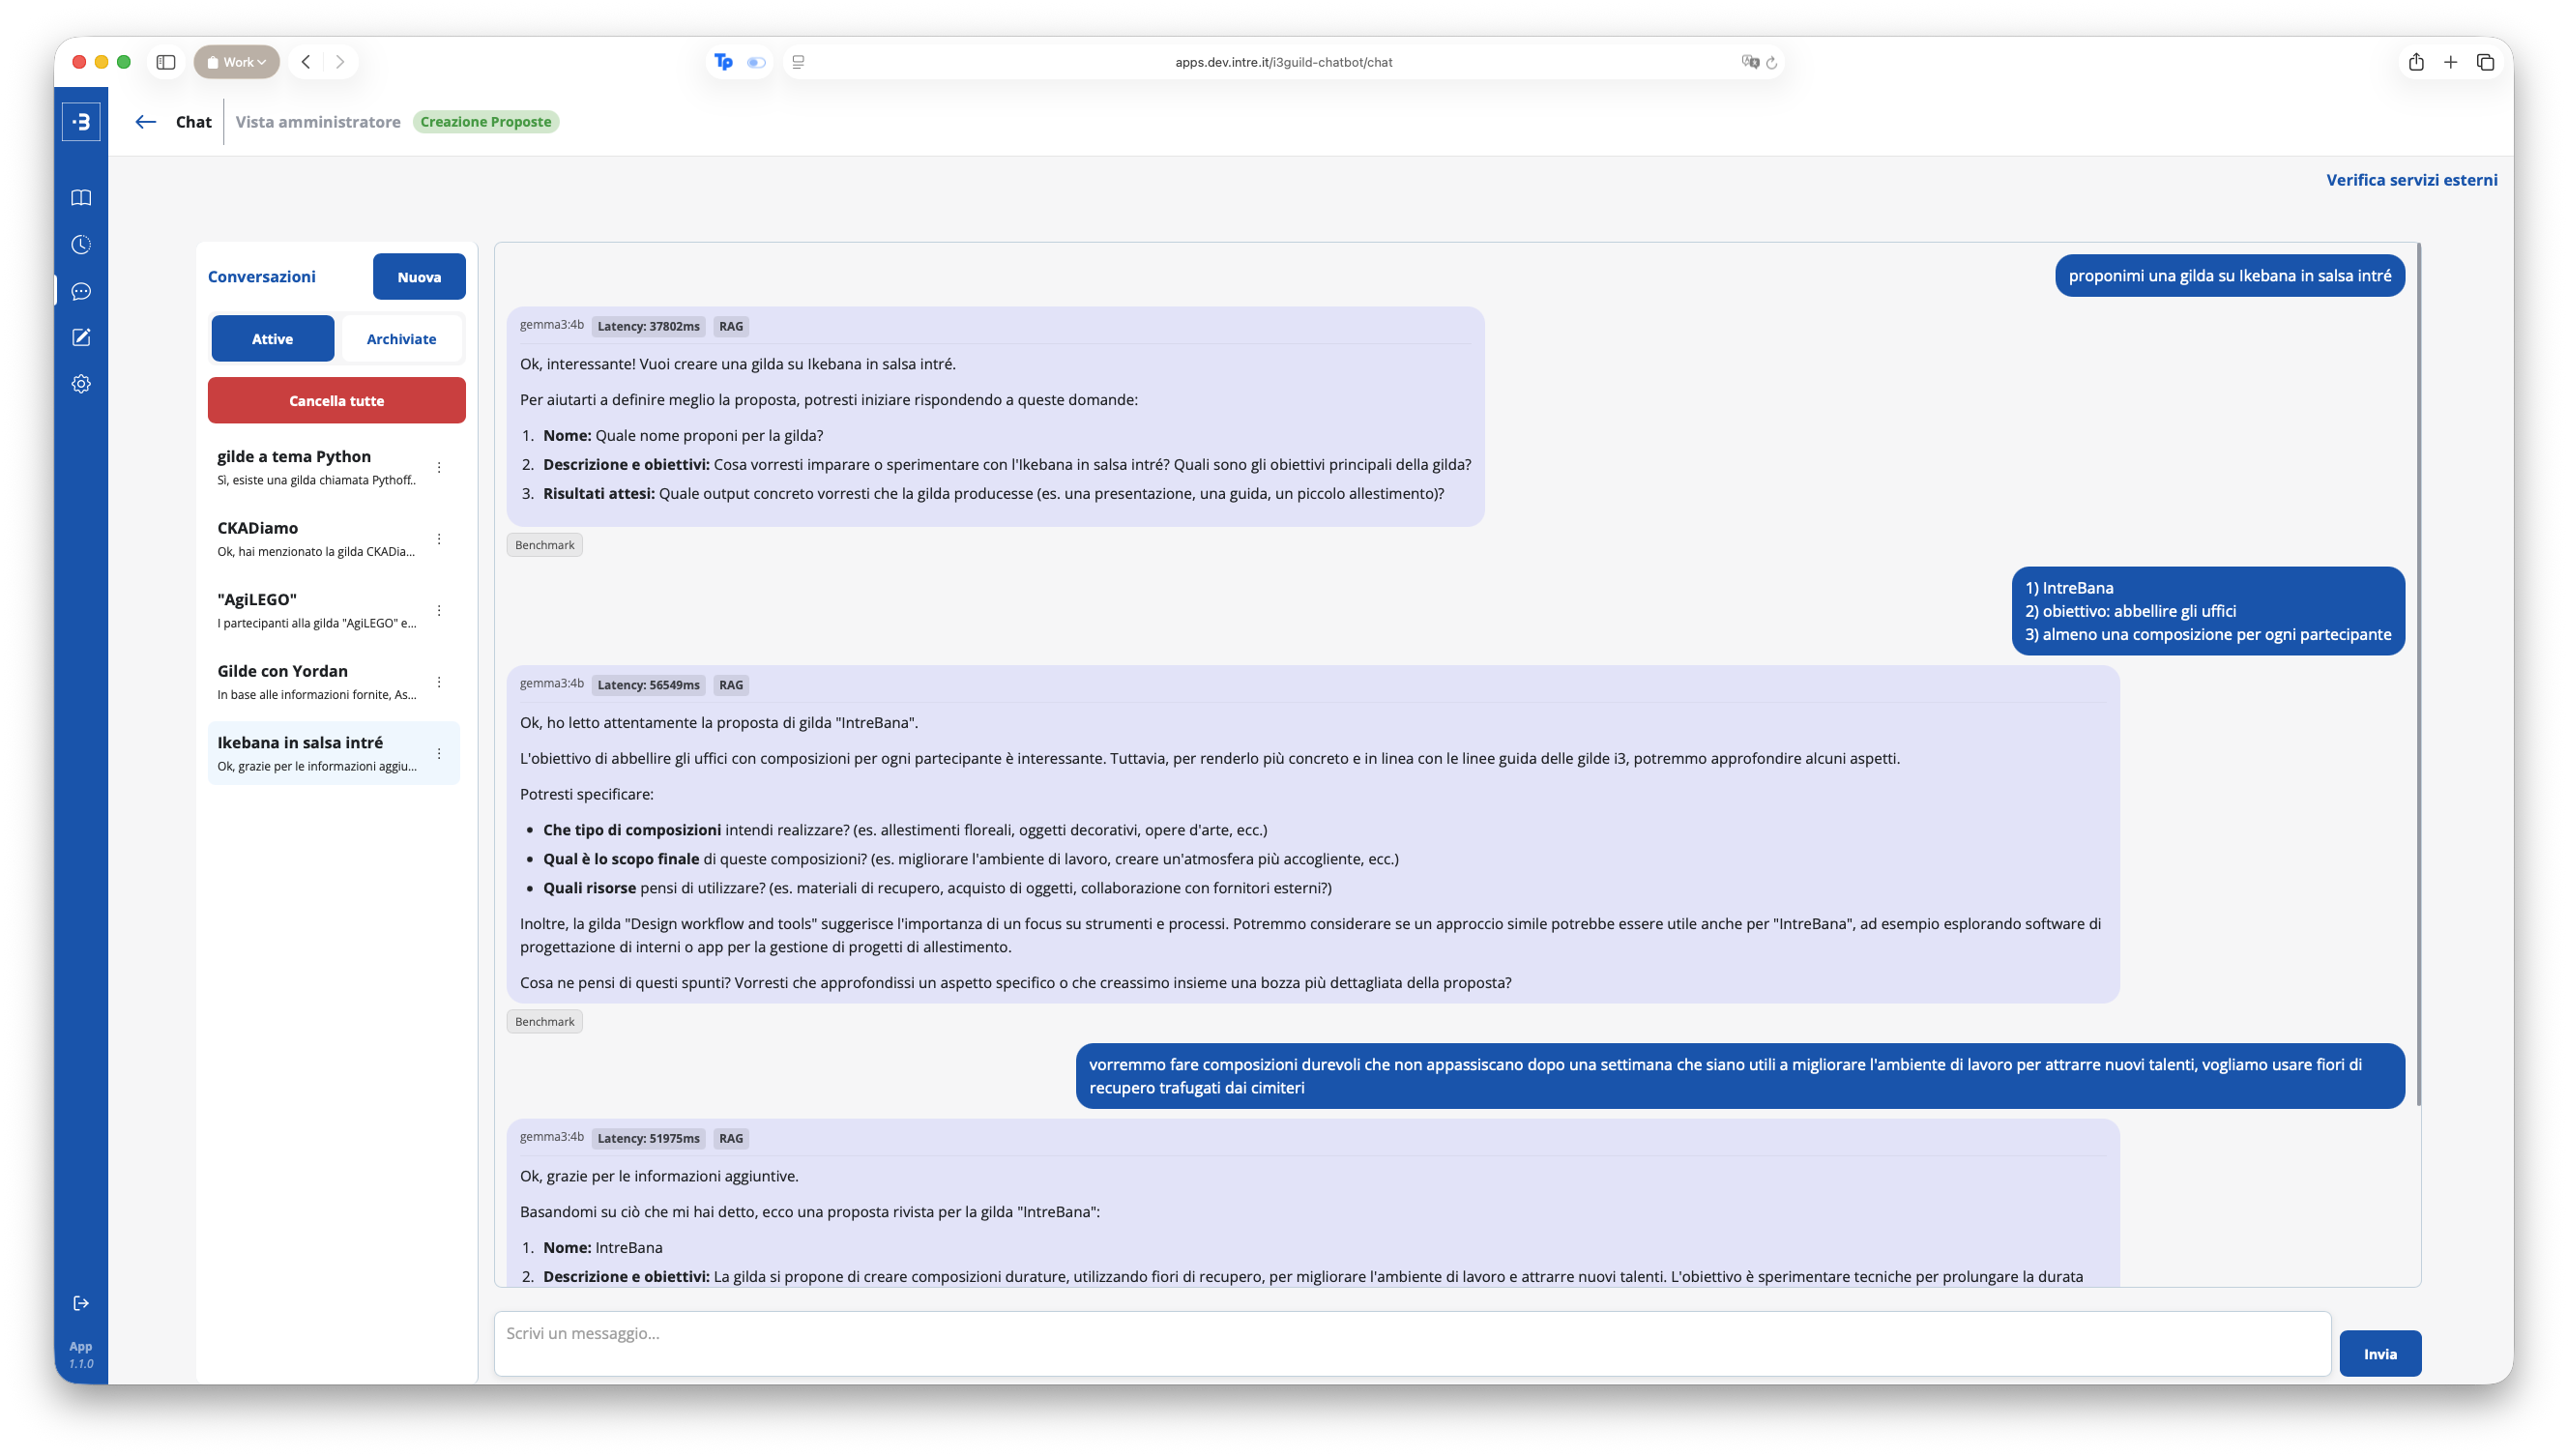
\includegraphics[width=0.95\textwidth]{chapter2/images/chat.png}
  \caption{Esempio di interazione con l'assistente RAG integrato in i3Guild.
    La schermata mostra la consultazione in linguaggio naturale del corpus e il
    collegamento tra risposta generata e informazioni recuperate.}
  \label{fig:i3guild_rag_screenshot}
\end{figure}

% -------------------------------------------------------------
\section{Requisiti di sistema}
\label{sec:system_requirements}
% -------------------------------------------------------------

Il caso d'uso appena descritto permette di passare dalla motivazione generale ai
requisiti del sistema. Essi sono stati ricavati dall'analisi del corpus, dai
vincoli infrastrutturali di Intré e dalle policy aziendali in materia di
protezione dei dati. La Tabella~\ref{tab:req_summary} sintetizza i requisiti ad
alto livello, suddivisi per categoria.

\begin{table}[ht]
  \centering
  \caption{Riepilogo requisiti ad alto livello.}
  \label{tab:req_summary}
  \small
  \begin{tabular}{p{3.5cm}p{9.5cm}}
    \toprule
    \textbf{Categoria} & \textbf{Requisiti principali} \\
    \midrule
    Funzionali & Ricerca semantica full-text su documenti interni; generazione
      di risposte contestualizzate con riferimenti alle fonti; capacità di
      filtraggio per metadati (epoca, modalità di partecipazione, proprietario
      della gilda). \\
    \addlinespace
    Privacy e conformità & Esecuzione on-premise; nessun invio di dati a
      servizi cloud esterni; logging e auditing degli accessi; protezione dei
      dati in conformità al GDPR~\cite{gdpr2016}. I rischi relativi alla
      privacy nei sistemi RAG, tra cui la possibile estrazione dei dati di
      retrieval, sono discussi in letteratura~\cite{zeng2024privacy}; la
      scelta on-premise costituisce la principale misura mitigativa adottata. \\
    \addlinespace
    Performance & Latenza compatibile con uso interattivo per query semplici,
      distinguendo tra modello già caricato e cold start; throughput adeguato a
      carichi concorrenti moderati; inferenza CPU-only come scenario primario. \\
    \addlinespace
    Costi e sostenibilità & Minimizzazione dei costi operativi tramite uso
      efficiente delle risorse (quantizzazione dei modelli, inferenza CPU);
      adozione di soluzioni open-source senza costi per licenze. \\
    \addlinespace
    Manutenibilità & Componenti modulari con interfacce standardizzate;
      automazione della pipeline di ingestione; documentazione e test
      automatizzati. \\
    \bottomrule
  \end{tabular}
\end{table}

\subsection{Vincoli architetturali}
\label{subsec:constraints}

I requisiti precedenti si traducono in vincoli architetturali non negoziabili.
L'esecuzione on-premise è il vincolo più rilevante: i dati delle Gilde, incluse
le informazioni sui partecipanti e sui progetti, non possono transitare su
infrastrutture cloud di terze parti. Il deployment locale diventa quindi la
condizione tecnica per rispettare i principi di integrità e riservatezza
previsti dal GDPR~\cite{gdpr2016}. L'integrazione deve inoltre rimanere
compatibile con lo stack i3Guild esistente, basato su Docker Compose,
PostgreSQL/Prisma, Next.js e Keycloak per l'autenticazione.

Un vincolo meno visibile, ma altrettanto determinante, riguarda le risorse
hardware. L'ambiente Docker dispone di 8~GB di RAM complessivi, condivisi tra
database, servizi applicativi, pipeline di embedding quando attiva e modello di
generazione del testo. Questa disponibilità limita la scelta del modello LLM,
discussa nella Sezione~\ref{subsec:llm_choice}, e impone di evitare componenti
con requisiti di memoria elevati. Per la stessa ragione, generazione ed
embedding devono restare locali senza fare affidamento su API esterne: Ollama
gestisce il modello generativo, mentre FastEmbed/Haystack produce gli embedding
senza dipendere da provider cloud.

% -------------------------------------------------------------
\section{Scelte tecnologiche e confronto}
\label{sec:tech_choices}
% -------------------------------------------------------------

Le scelte tecnologiche sono state effettuate a partire dai vincoli appena
definiti. Per ciascun componente principale dello stack sono state valutate
alternative compatibili con l'esecuzione on-premise, privilegiando soluzioni
semplici da integrare nello stack i3Guild, osservabili e sostenibili rispetto
alle risorse disponibili.

\subsection{Framework di orchestrazione RAG}
\label{subsec:framework_choice}

Il framework di orchestrazione deve collegare ingestione, embedding, retrieval
e generazione senza introdurre eccessiva complessità operativa. Sono stati
considerati tre framework open-source: \textbf{LangChain},
\textbf{LlamaIndex} e \textbf{Haystack~2.x}.

\paragraph{LangChain} offre l'ecosistema più ampio di integrazioni e una forte
vocazione verso workflow agentici e \textit{multi-step reasoning}. LangGraph ha
ampliato questa impostazione, permettendo di modellare applicazioni multi-agente
come grafi di stato. Tale flessibilità è utile in scenari complessi, ma nel progetto
in esame introduce un costo non trascurabile in termini di curva di
apprendimento, stabilità delle API e manutenzione, anche alla luce dei
\textit{breaking changes} frequenti.

\paragraph{LlamaIndex} è orientato alla gestione dei dati e al retrieval
avanzato. Offre numerosi data connector e strutture di indicizzazione
specializzate, risultando particolarmente adatto a pipeline di
question-answering documentale. Rispetto al caso
considerato, tuttavia, l'obiettivo principale non è solo indicizzare sorgenti
eterogenee, ma integrare una pipeline osservabile e facilmente testabile nello
stack applicativo esistente.

\paragraph{Haystack 2.x} (deepset) adotta un modello a componenti tipizzati
con input/output espliciti, organizzati in pipeline dichiarative serializzabili
in YAML. La sua politica pipeline-first favorisce la tracciabilità, i test e
la sostituzione dei componenti in produzione, aspetti più rilevanti per il
prototipo rispetto alla disponibilità di astrazioni agentiche avanzate.
La Tabella~\ref{tab:framework_comparison} sintetizza il confronto tra i tre
framework considerati rispetto ai criteri più rilevanti per il prototipo.

\begin{table}[ht]
  \centering
  \caption{Confronto sintetico dei framework RAG candidati.}
  \label{tab:framework_comparison}
  \small
  \begin{tabularx}{\textwidth}{L{2.8cm}YYY}
    \toprule
    \textbf{Criterio} & \textbf{LangChain} & \textbf{LlamaIndex} &
      \textbf{Haystack 2.x} \\
    \midrule
    Filosofia & Agente/imperativa & Data-first & Pipeline dichiarativa \\
    Orientamento operativo & Workflow agentici e catene applicative &
      Indicizzazione e gestione dati & Pipeline RAG dichiarative \\
    Integrazione Qdrant & Nativa & Nativa & Nativa \\
    Integrazione Ollama & Sì & Sì & Sì \\
    Testabilità pipeline & Media & Media & Alta \\
    Serializzazione YAML & No & Parziale & Sì \\
    Adatto per produzione RAG & Sì (con overhead) & Sì & Sì (preferito) \\
    \bottomrule
  \end{tabularx}
\end{table}

\noindent Alla luce di questo confronto, Haystack 2.x risulta la soluzione più
coerente con il progetto. L'architettura a componenti tipizzati, la
documentazione rigorosa, le integrazioni native con Qdrant
(\texttt{QdrantDocumentStore}), FastEmbed per embedding densi e sparsi e Ollama
per la generazione permettono di costruire una pipeline osservabile senza
introdurre un framework agentico più complesso del necessario. La possibilità di
serializzare le pipeline rafforza questa scelta in un sistema RAG orientato alla
produzione e vincolato all'esecuzione on-premise.

\subsection{Database vettoriale}
\label{subsec:vectordb_choice}

La ricerca di similarità approssimata (\emph{Approximate Nearest Neighbor},
ANN) su vettori ad alta dimensionalità è il componente infrastrutturale che
abilita il retrieval. La scelta del database vettoriale incide su latenza,
filtraggio per metadati, semplicità di deployment e capacità di manutenzione
dell'indice; per questo sono stati valutati quattro database vettoriali
self-hostable.
La Tabella~\ref{tab:vectordb_comparison} mostra il confronto usato per
motivare la scelta di Qdrant.

\begin{table}[ht]
  \centering
  \caption{Analisi comparativa dei database vettoriali candidati.}
  \label{tab:vectordb_comparison}
  \small
  \begin{tabularx}{\textwidth}{L{1.5cm}L{1.5cm}L{1.4cm}YYY}
    \toprule
    \textbf{Database} & \textbf{Impl.} & \textbf{Indice} &
      \textbf{Filtering} & \textbf{Dashboard} & \textbf{Deployment} \\
    \midrule
    \textbf{Qdrant} & Rust & HNSW & Pre-filtering payload & Web UI &
      1 container \\
    pgvector & C & IVFFlat / HNSW & SQL \texttt{WHERE} & No &
      Estensione PG \\
    Milvus & Go/C++ & HNSW, IVF & Attribute-based & Attu &
      Multi-container \\
    Chroma & Python & HNSW (hnswlib) & Metadata base & No & 1 container \\
    \bottomrule
  \end{tabularx}
\end{table}

Il confronto non si limita alle prestazioni pure: nel contesto i3Guild hanno
peso anche la semplicità operativa e la possibilità di applicare filtri sui
metadati delle Gilde. I principali criteri di esclusione e selezione sono i
seguenti:

\begin{itemize}
  \item \textbf{pgvector} è stato considerato in quanto l'infrastruttura
    i3Guild utilizza già PostgreSQL. Tuttavia, la letteratura segnala che le
    prestazioni di pgvector degradano significativamente oltre le centinaia di
    migliaia di vettori, con ritardi fino a 15 volte superiori rispetto a
    Qdrant in termini di throughput su dataset grandi. In questo progetto hanno
    pesato soprattutto l'assenza di una dashboard integrata e di un payload
    filtering flessibile, che avrebbero reso meno diretta la gestione dei
    metadati delle Gilde.
  \item \textbf{Milvus} è stato escluso per l'elevata complessità di deploy:
    richiede componenti aggiuntivi (\texttt{etcd}, \texttt{MinIO}), aumentando
    il carico operativo incompatibile con i vincoli del progetto.
  \item \textbf{Chroma} è implementato in Python e soffre di instabilità della
    persistenza dati nelle versioni precedenti; è più adatto a prototipi
    che a sistemi di produzione.
  \item \textbf{Qdrant} è scritto in Rust e offre buone prestazioni con latenze
    stabili nei benchmark disponibili. La funzionalità di pre-filtering, che
    applica i filtri sui payload \emph{prima} della ricerca vettoriale, è
    particolarmente rilevante per query
    contestuali come ``gilda dell'epoca X'': il filtering riduce lo spazio di
    ricerca prima del calcolo ANN, mantenendo il top-$K$ accurato. Offre Web
    UI integrata su porta 6333, client TypeScript ufficiale compatibile con
    Next.js e deploy in singolo container Docker.
\end{itemize}

\noindent Per le ragioni discusse, e in particolare per il bilanciamento tra
prestazioni, semplicità di deployment e supporto al filtering sui metadati,
Qdrant è stato selezionato come database vettoriale del progetto. La scelta è
coerente con il vincolo aziendale di self-hosting e con la necessità di
mantenere il sistema manutenibile anche in un contesto prototipale.

\subsection{Modello di embedding}
\label{subsec:embedding_choice}

Il modello di embedding converte i documenti testuali in rappresentazioni
numeriche interrogabili da Qdrant. Nel progetto questa funzione è separata
dall'inferenza generativa: Ollama serve il modello di chat, mentre FastEmbed,
tramite Haystack, produce le rappresentazioni usate per l'indicizzazione. La
pipeline genera sia embedding densi sia embedding sparsi, così il retrieval può
combinare similarità semantica e corrispondenza lessicale su nomi propri,
tecnologie e termini ricorrenti nelle Gilde.

\begin{table}[ht]
  \centering
  \caption{Configurazione embedding del sistema RAG.}
  \label{tab:embedding_models}
  \small
  \begin{tabular}{L{2.7cm}L{4.1cm}L{3cm}L{3.6cm}}
    \toprule
    \textbf{Ruolo} & \textbf{Componente Haystack} & \textbf{Default} &
      \textbf{Funzione} \\
    \midrule
    Embedding denso & Document/text embedder denso &
      \makecell[l]{\texttt{paraphrase-}\\\texttt{multilingual-}\\\texttt{mpnet-base-v2}} &
      Similarità semantica tra query e documenti. \\
    Embedding sparso & Document/text embedder sparso & \makecell[l]{\texttt{prithivida/}\\\texttt{Splade\_PP\_en\_v1}} &
      Matching lessicale pesato, utile per termini specifici. \\
    Store ibrido & \breakcode{QdrantDocumentStore} con
      \breakcode{use_sparse_embeddings=true} & \breakcode{i3guild_knowledge} &
      Persistenza con vettori densi e rappresentazioni sparse. \\
    \bottomrule
  \end{tabular}
\end{table}

\noindent La separazione tra indicizzazione e generazione riduce
l'accoppiamento operativo: Ollama rimane dedicato alla risposta LLM, mentre il
job batch produce gli embedding senza dipendere dal server di chat. La
componente sparsa rende inoltre il retrieval meno dipendente dalla sola
similarità densa, aspetto rilevante in un corpus dove nomi propri, tecnologie e
termini ricorrenti hanno spesso valore informativo letterale. Ingestione e query
seguono quindi lo stesso schema operativo: in scrittura vengono generati
embedding densi e sparsi dei documenti; in lettura la query viene trasformata
nelle due rappresentazioni corrispondenti e inviata al retriever ibrido Qdrant.
Il valore
\texttt{EMBEDDING\_DIMENSIONS=768} rimane il riferimento per la componente
densa.

La scelta della ricerca ibrida non deriva da una valutazione quantitativa
condotta sul corpus i3Guild, perché durante il progetto non è stato costruito
un dataset annotato con query e documenti rilevanti. È però coerente con
evidenze esterne recenti: nei task RAG di TREC 2025 un sistema sparse+dense con
reranking ottiene i migliori risultati riportati dal team NITATREC
(\textit{MAP} 0.1037, \textit{nDCG@30} 0.527 e \textit{Recall@100}
0.158)~\cite{sinha2025nitatrec}; in un benchmark finanziario su documenti misti
testo-tabella, una pipeline a due stadi con retrieval ibrido e reranking
raggiunge \textit{Recall@5} 0.816 e \textit{MRR@3} 0.605, superando i metodi
single-stage~\cite{akarsu2026bm25correctiverag}. Altri studi mostrano però che
il vantaggio non è universale: nel dominio biomedicale una baseline densa resta
molto competitiva e le differenze tra strategie dipendono dal corpus e dalle
metriche considerate~\cite{bal2026biomedicalretrieval}. Per i3Guild questi
risultati vanno quindi usati come supporto alla scelta progettuale, non come
prova sperimentale locale: la componente sparsa è motivata soprattutto dalla
presenza di nomi di Gilde, ruoli, modalità di partecipazione e termini tecnici
che hanno valore informativo letterale.

\subsection{Server di inferenza LLM e selezione del modello di chat}
\label{subsec:llm_choice}

Il componente di generazione del testo è gestito da \textbf{Ollama}, server di
inferenza locale che supporta modelli in formato GGUF e consente l'uso di
varianti quantizzate a 4 e 8 bit. Nel prototipo aziendale la scelta del modello
di chat è stata condizionata da un vincolo operativo preciso: l'intero stack
Docker dispone di risorse limitate e deve eseguire, nello stesso ambiente,
PostgreSQL, Qdrant, il servizio Next.js, la pipeline RAG e Ollama. Per questo
la selezione non mira a identificare il modello migliore in senso assoluto, ma
un modello sufficientemente stabile per validare l'integrazione end-to-end.

\noindent Il modello adottato nel prototipo è \texttt{gemma3:4b}, distribuito
in Ollama come \texttt{gemma3:latest}. La scelta deriva da prove preliminari
interne su modelli disponibili nel registry Ollama, valutati rispetto a latenza
percepita, consumo di memoria e qualità minima delle risposte in presenza di
contesto RAG. Il modello resta caricabile nello stesso ambiente dei servizi
PostgreSQL, Qdrant, Next.js e FastAPI, ma offre un margine qualitativo maggiore
rispetto a modelli da circa 1B parametri. Le risposte non sono usate come prova
generale della qualità del modello; sono sufficienti per validare il flusso
applicativo quando il contesto recuperato da Qdrant è pertinente.

Le prove locali hanno confrontato dodici modelli Ollama su 14 query, divise tra
prompt generali e prompt RAG. La valutazione manuale ha assegnato tre punteggi
per accuratezza o fedeltà, pertinenza e coerenza. I risultati non costituiscono
un benchmark scientifico, perché il numero di query è ridotto e il carico della
macchina non è stato isolato; sono però utili come criterio progettuale. In
media, \texttt{gemma3:1b} ha mostrato la latenza totale più bassa
(\(\approx 6.7\) s) e un buon throughput (\(\approx 28\) parole/s), ma una
coerenza più debole nelle risposte RAG. \texttt{gemma3:4b} ha richiesto più
tempo (\(\approx 17.3\) s in media), mantenendo però il punteggio medio più alto
tra i modelli di dimensione compatibile con il prototipo. Modelli ragionativi
come \texttt{phi4-mini-reasoning} hanno prodotto latenze troppo elevate per
l'uso interattivo, mentre alcune alternative molto compatte hanno mostrato
output meno controllabili. La scelta di \texttt{gemma3:4b} privilegia quindi un
compromesso pratico: qualità sufficiente, integrazione immediata in Ollama e
risorse ancora compatibili con l'ambiente condiviso.

\noindent Questa valutazione resta volutamente interna al progetto aziendale:
serve a rendere eseguibile il prototipo i3Guild, non a produrre conclusioni
generali sull'inferenza locale. La generalizzazione del problema, cioè la misura
sistematica di memoria, cold start, \emph{time-to-first-token}, throughput e
impatto della quantizzazione su Apple Silicon, viene affrontata nei
Capitoli~\ref{chap:ottimizzazione} e~\ref{chap:evaluation}.

% -------------------------------------------------------------
\section{Proposta architetturale}
\label{sec:architecture}
% -------------------------------------------------------------

Le scelte tecnologiche descritte portano a un'architettura modulare e
containerizzata, in cui ingestione e normalizzazione dei dati, generazione degli
embedding, persistenza vettoriale, retrieval e inferenza tramite LLM restano
fasi operative distinte. Questa separazione rende i componenti più facili da
monitorare e sostituire, mantenendo l'integrazione coerente con lo stack
i3Guild. La Figura~\ref{fig:architecture} mostra lo schema generale
dell'architettura.

\begin{figure}[ht]
  \centering
  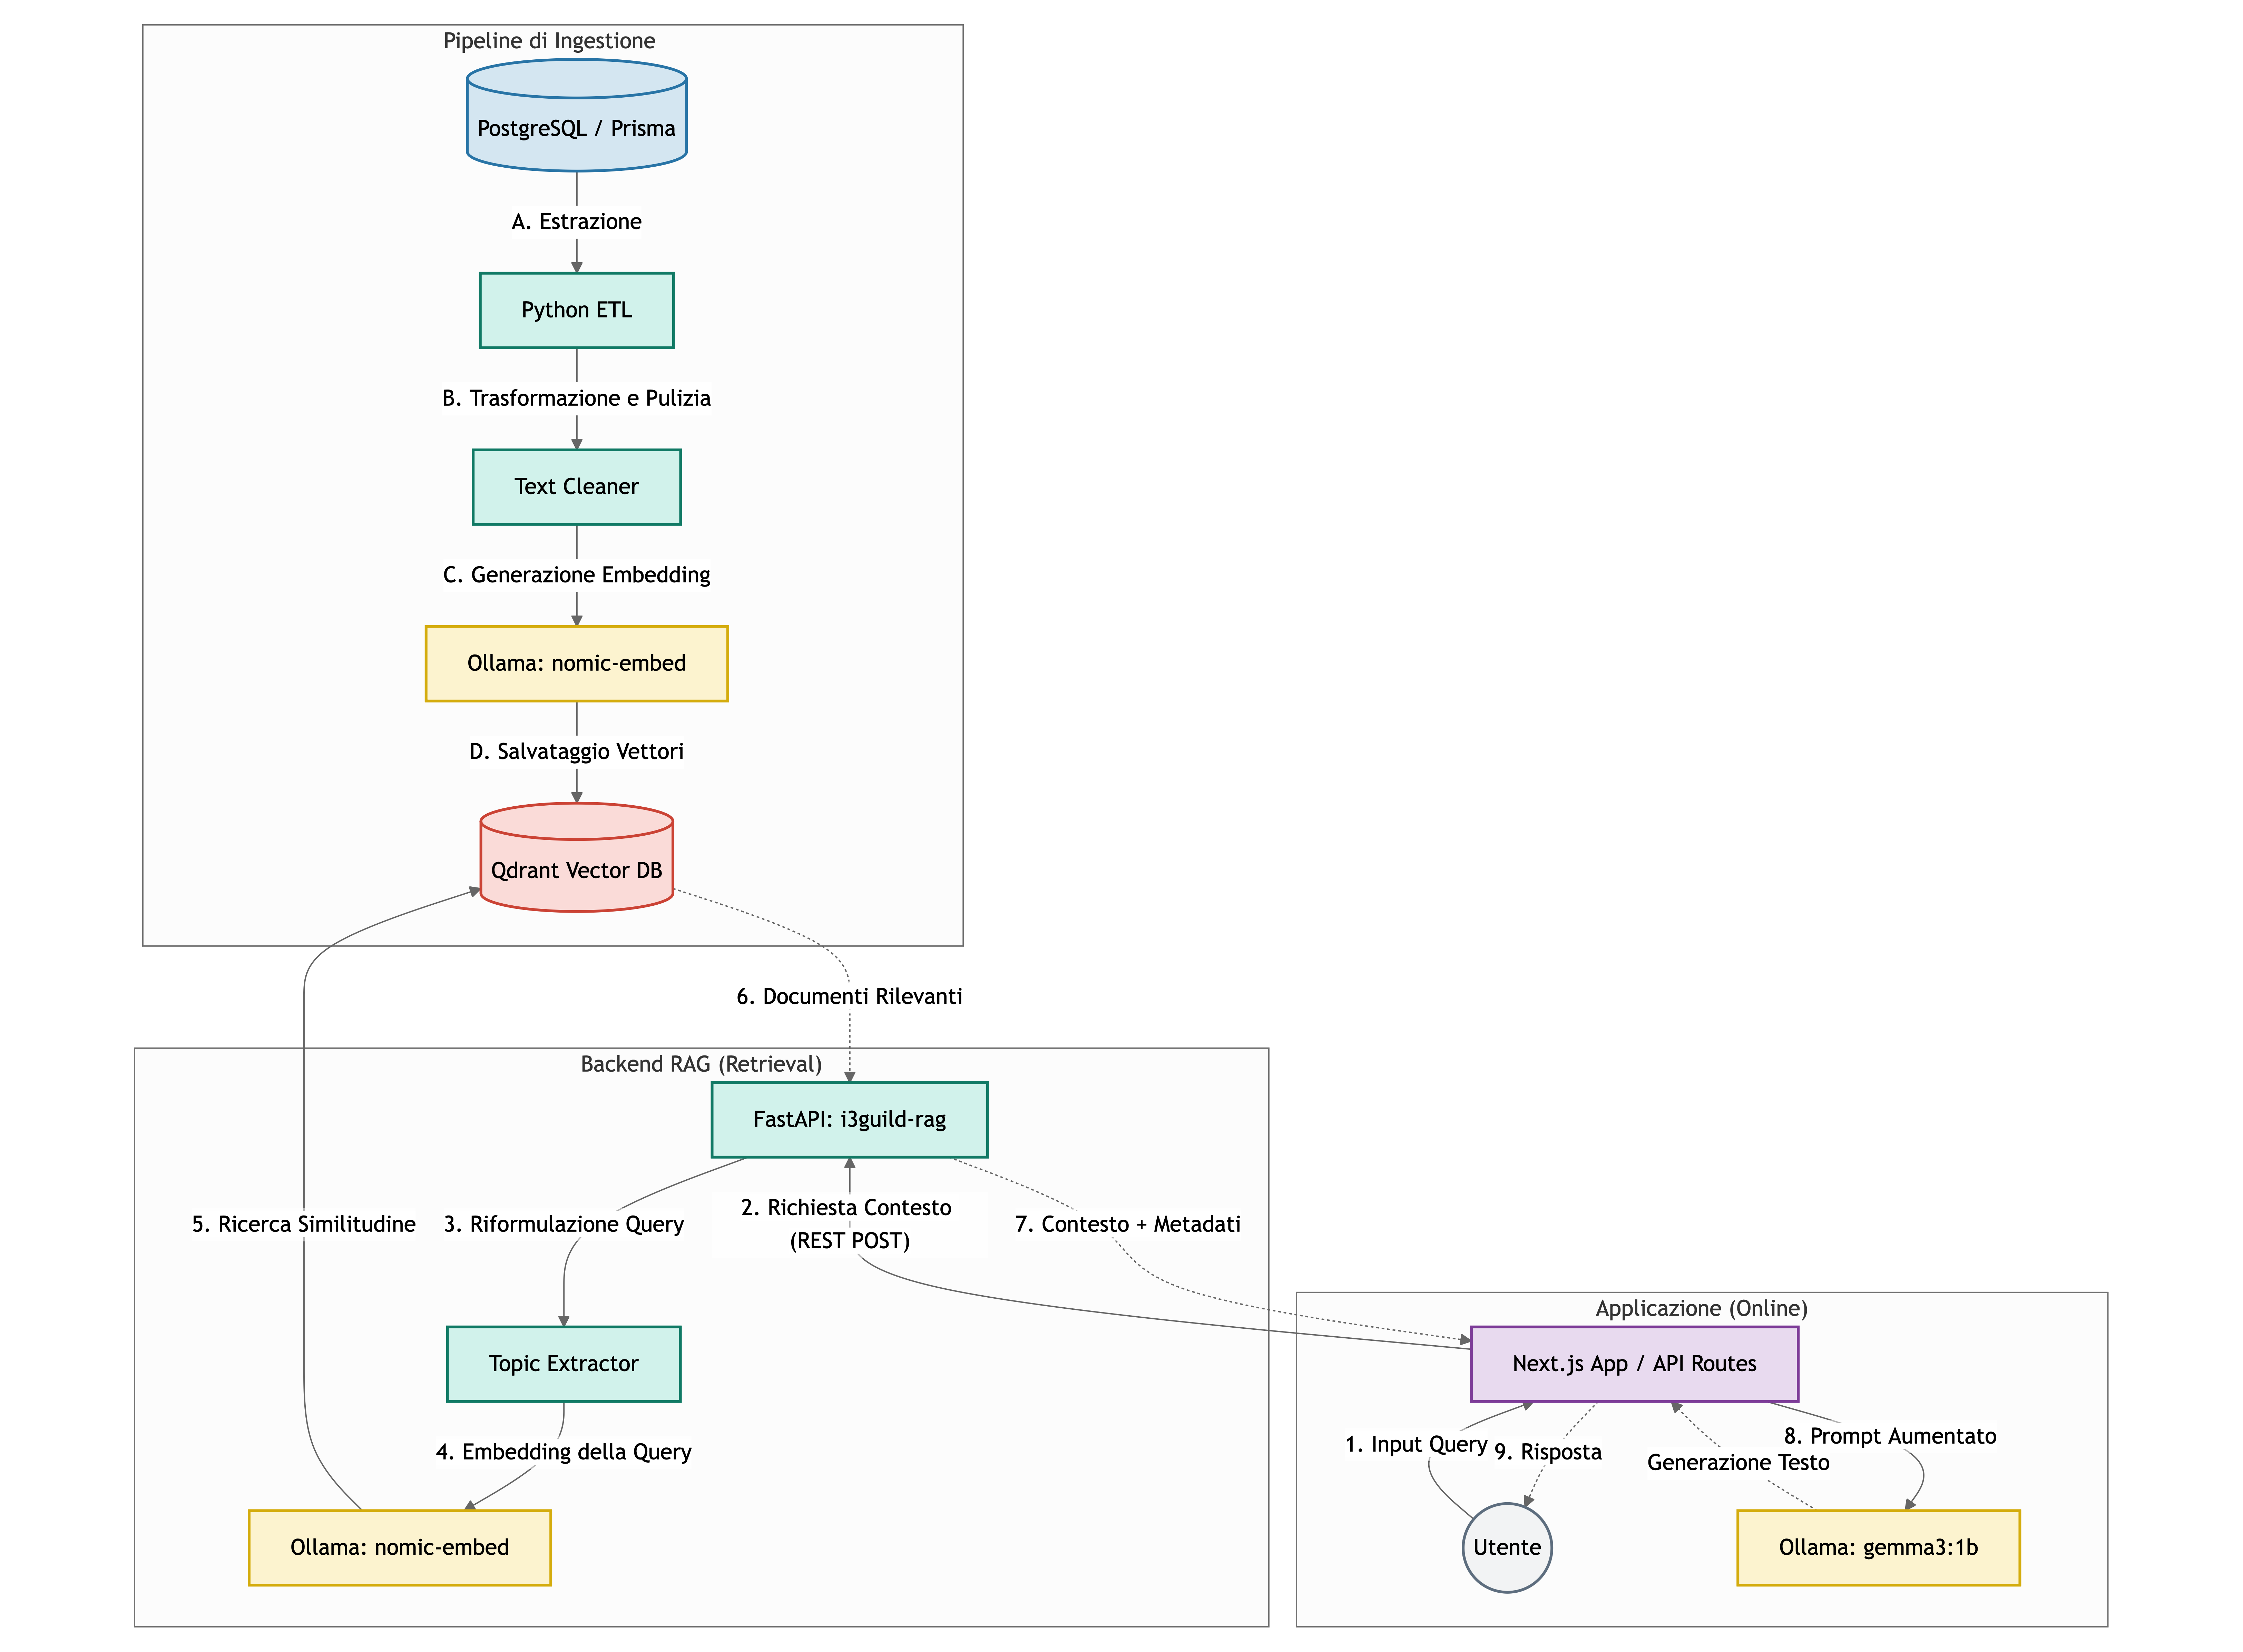
\includegraphics[width=0.85\textwidth]{chapter2/images/architecture_diagram.png}
  \caption{Schema architetturale del sistema RAG on-premise per i3Guild.
    Il flusso di ingestione (ETL) popola Qdrant a partire da PostgreSQL;
    il flusso di retrieval serve le query di Next.js tramite FastAPI.}
  \label{fig:architecture}
\end{figure}

\subsection{Componenti principali}
\label{subsec:components}

I componenti non sono separati soltanto per ragioni di deployment: ciascuno
risponde a un requisito emerso nelle sezioni precedenti. PostgreSQL rimane la
sorgente autoritativa dei dati; Qdrant rende interrogabile il corpus per
similarità; Ollama consente di mantenere la generazione in locale; FastAPI
espone verso Next.js un confine applicativo chiaro, senza incorporare la logica
RAG direttamente nel frontend.

\begin{description}
  \item[Ingestione e pre-processing]
    Pipeline batch Python che esegue le fasi ETL descritte nella
    Sezione~\ref{subsec:ingestion_pipeline}. Acquisisce i documenti da
    PostgreSQL, normalizza il testo, esegue il chunking, genera embedding densi
    e sparsi con FastEmbed/Haystack e indicizza su Qdrant.

  \item[Strategia di chunking] Sulla base dell'analisi dei dati
    (Sezione~\ref{subsec:data_analysis}), viene adottato l'approccio a
    \emph{documento consolidato} (1 Gilda $\leftrightarrow$ 1 documento
    vettoriale): tutti i campi testuali rilevanti sono concatenati in un unico
    documento con separatori strutturati. Per gli outlier che superano il limite
    configurato viene applicato chunking con overlap, mantenendo nel chunk
    l'intestazione della Gilda. Questo approccio preserva il contesto semantico
    nella maggior parte dei casi e mantiene gestibili upsert e cancellazioni su
    Qdrant.

  \item[Database vettoriale (Qdrant)] Collection principale
    \texttt{i3guild\_knowledge} configurata per retrieval ibrido: vettore denso
    a 768 dimensioni, rappresentazione sparsa e payload JSON con metadati
    indicizzati per il filtering (Sezione~\ref{subsec:qdrant_collection}).

  \item[Orchestrazione RAG (Haystack 2.x)] Haystack è usato sia nel job di
    indicizzazione sia nel servizio di query. La pipeline batch collega gli
    embedder densi e sparsi con il writer; la pipeline di query usa i
    componenti corrispondenti e il retriever ibrido Qdrant.

  \item[Inference LLM (Ollama)] Server di inferenza locale; modello di chat
    adottato: \texttt{gemma3:4b}, selezionato sulla base di prove preliminari
    coerenti con i vincoli del prototipo
    (Sezione~\ref{subsec:llm_choice}).

  \item[Servizio API (FastAPI)] Microservizio Python che espone endpoint di
    retrieval e generazione, tra cui \texttt{POST /rag/retrieve} (porta 8000,
    mappata a 8002 su host). Restituisce documenti con score di similarità e
    campi diagnostici.

  \item[Osservabilità e sicurezza] Logging centralizzato, metriche di latenza
    e utilizzo risorse; autenticazione tramite Keycloak (già presente in
    i3Guild); cifratura a riposo per i dataset sensibili.
\end{description}

\subsection{Progettazione della collection Qdrant}
\label{subsec:qdrant_collection}

La collection \texttt{i3guild\_knowledge} è il punto in cui la conoscenza
estratta da i3Guild viene trasformata in indice interrogabile. La configurazione,
riportata nella Tabella~\ref{tab:qdrant_config}, supporta retrieval ibrido:
similarità vettoriale densa e componente sparsa nello stesso store.

\begin{table}[ht]
  \centering
  \caption{Parametri di configurazione della collection Qdrant.}
  \label{tab:qdrant_config}
  \small
  \begin{tabular}{L{4.2cm}L{3.5cm}L{5.5cm}}
    \toprule
    \textbf{Parametro} & \textbf{Valore} & \textbf{Motivazione} \\
    \midrule
    \breakcode{embedding_dim} & 768 & Dimensione della componente densa FastEmbed \\
    \breakcode{vectors.distance} & \breakcode{Cosine} & Standard per similarità
      semantica testuale \\
    \breakcode{use_sparse_embeddings} & \breakcode{true} & Abilita la componente
      sparsa per retrieval ibrido \\
    \breakcode{recreate_index} & \breakcode{true} (job batch) & Ricrea la
      collection ibrida mantenendo lo stesso nome \\
    \breakcode{hnsw_config.m} & 16 (default) & Compromesso velocità/precisione \\
    \breakcode{hnsw_config.ef_construct} & 100 (default) & Qualità dell'indice
      in fase di build \\
    \bottomrule
  \end{tabular}
\end{table}

Ogni punto nella collection porta un payload JSON con i campi elencati nella
Tabella~\ref{tab:qdrant_payload}, in particolare i campi marcati come indicizzati abilitano il
pre-filtering, caratteristica distintiva di Qdrant che applica i filtri sul
payload \emph{prima} della ricerca vettoriale, garantendo che il calcolo del
top-$K$ sia effettuato solo sul sottoinsieme filtrato.

\begin{table}[ht]
  \centering
  \caption{Struttura del payload Qdrant per la collection
    \texttt{i3guild\_knowledge}.}
  \label{tab:qdrant_payload}
  \small
  \begin{tabular}{L{3.7cm}L{2cm}L{5.8cm}L{1.4cm}}
    \toprule
    \textbf{Campo} & \textbf{Tipo} & \textbf{Descrizione} &
      \makecell[l]{\textbf{Ind.}} \\
    \midrule
    \breakcode{guild_id} & integer & ID della gilda sorgente & Sì \\
    \breakcode{guild_name} & keyword & Nome della gilda & Sì \\
    \breakcode{epoch_id} & integer & ID dell'epoca di appartenenza & Sì \\
    \breakcode{epoch_start} & datetime & Data inizio epoca & Sì \\
    \breakcode{epoch_end} & datetime & Data fine epoca (nullable) & Sì \\
    \breakcode{participation_mode} & keyword & FullRemote / Hybrid / OnSite & Sì \\
    \breakcode{is_individual} & bool & Gilda individuale & Sì \\
    \breakcode{owner_id} & keyword & ID del proprietario & Sì \\
    \breakcode{participants} & keyword[] & Nomi dei partecipanti & Sì \\
    \breakcode{participant_count} & integer & Numero di partecipanti & No \\
    \breakcode{source_text} & text & Testo originale del chunk & No \\
    \breakcode{last_synced} & datetime & Timestamp ultima sincronizzazione & No \\
    \bottomrule
  \end{tabular}
\end{table}

Gli ID dei documenti sono deterministici nel formato
\texttt{guild-\{guild\_id\}-chunk-\{index\}}. La reindicizzazione della stessa
Gilda produce quindi gli stessi identificativi e consente a Qdrant di
sovrascrivere i punti esistenti quando la policy è
\texttt{DuplicatePolicy.OVERWRITE}.

\subsection{Pipeline di ingestione ETL}
\label{subsec:ingestion_pipeline}

La pipeline ETL ha il compito di mantenere allineata la rappresentazione
vettoriale con i dati applicativi. Il job batch esegue le seguenti fasi:

\begin{enumerate}
  \item \textbf{Extract}: connessione a PostgreSQL e query SQL con JOIN su
    \texttt{Epoch}, \texttt{GuildUserRelation} ed \texttt{ExternalUser} per
    estrarre tutti i campi semantici delle Gilde insieme ai nomi dei
    partecipanti.
  \item \textbf{Transform}: normalizzazione HTML tramite \texttt{BeautifulSoup},
    composizione di documenti Haystack con sezioni marcate e chunking con
    overlap quando il testo supera il limite configurato.
  \item \textbf{Embed}: generazione di embedding densi tramite
    \texttt{FastembedDocumentEmbedder} e di embedding sparsi tramite
    \texttt{FastembedSparseDocumentEmbedder}.
  \item \textbf{Load}: scrittura su Qdrant tramite \texttt{DocumentWriter} con
    policy configurabile, di default \texttt{DuplicatePolicy.OVERWRITE}.
\end{enumerate}

La struttura della pipeline Haystack è riportata in Appendice~\ref{app:B},
Listato~\ref{lst:ingest_pipeline}.

Il container della pipeline mantiene comportamento batch: esegue ingestione,
upsert su Qdrant e termina con codice 0 in caso di successo o 1 in caso di
errore. Questa separazione evita che indicizzazione e query interattive
competano nello stesso processo.

\subsection{Pipeline di retrieval e logica di ranking}
\label{subsec:retrieval_pipeline}

La pipeline di retrieval usa l'indice ibrido Qdrant per recuperare i documenti
più pertinenti alla query e restituisce al livello applicativo un contesto già
filtrato. La query viene trasformata sia in embedding denso sia in embedding
sparso; le due rappresentazioni alimentano \texttt{QdrantHybridRetriever}. Il
sistema non adotta un valore
\texttt{top\_k} fisso: una soglia rigida rischierebbe infatti di includere
documenti marginali nelle query semplici o di tagliare informazioni utili nelle
query più ampie. Per questo viene applicato un approccio adattivo in tre stadi:

\begin{enumerate}
  \item \textbf{Soglia di similarità} (default: cosine score $\geq 0.5$):
    esclude documenti semanticamente non pertinenti.
  \item \textbf{Rilevamento del calo relativo}: se la caduta percentuale tra
    due score consecutivi supera una soglia configurabile (default: 0.08), la
    lista viene troncata al confine naturale della rilevanza.
  \item \textbf{Cap di sicurezza} (default: $\leq 5$ documenti): limite
    massimo per controllare la dimensione del contesto passato al modello
    generativo.
\end{enumerate}

Prima del taglio finale viene applicata una deduplicazione post-retrieval: il
servizio rimuove documenti ripetuti per ID, fingerprint testuale e similarità
fuzzy. Una cache in-process con TTL breve riduce inoltre richieste ripetute con
stessi parametri, senza cambiare il modello dati persistente.

\subsubsection{Query rewriting e Topic-First Search}
\label{subsubsec:query_rewriting}

Nel contesto i3Guild, molte query contengono parole ricorrenti come ``gilda'',
``fondare'' o ``consigli''. Questi termini descrivono l'interazione con il
sistema, ma non il tema informativo cercato; se mantenuti nella query, possono
dominare lo spazio degli embedding e produrre risultati generici. Il
\emph{query rewriting}, discusso anche in framework come
RQ-RAG~\cite{chan2024rqrag}, viene quindi utilizzato per isolare il topic
rilevante prima del retrieval. L'approccio implementato tramite la funzione
\texttt{extract\_topic\_query()} opera in tre passaggi:

\begin{enumerate}
  \item Normalizzazione e rimozione della punteggiatura.
  \item Filtraggio di un insieme esplicito di \emph{domain stopwords}
    (\texttt{DOMAIN\_STOPWORDS}), unito alle stopwords italiane generiche.
  \item Estrazione dei token residui, preservando gli acronimi scritti in
    maiuscolo quando hanno lunghezza compresa tra due e cinque caratteri.
\end{enumerate}

Il risultato non è una riscrittura semantica della domanda, ma una riduzione
lessicale. Se la stringa estratta non è vuota ed è diversa dalla query originale
normalizzata, il retrieval la usa come query di ricerca, altrimenti
mantiene la query originale. La Tabella~\ref{tab:query_rewriting} riporta alcuni
esempi.

\begin{table}[ht]
  \centering
  \caption{Effetto del query rewriting su esempi di query utente.}
  \label{tab:query_rewriting}
  \small
  \begin{tabular}{cc}
    \toprule
    \textbf{Query originale} & \textbf{Topic estratto}\\
    \midrule
    ``vorrei fondare una gilda sulla musica'' &
      \texttt{musica} \\
    ``intelligenza artificiale'' & \texttt{intelligenza artificiale} \\
    ``Partecipanti al progetto di design'' &
      \texttt{partecipanti progetto design} \\
    ``quali gilde si occupano di AI?'' &
      \texttt{occupano ai}\\
    \bottomrule
  \end{tabular}
\end{table}

\subsection{Endpoint API di riferimento}
\label{subsec:api_endpoint}

Il risultato della pipeline viene esposto tramite un endpoint FastAPI, che
costituisce il contratto tra il servizio RAG e l'applicazione Next.js.
L'endpoint principale è il seguente:

\noindent \textbf{POST} \texttt{/rag/retrieve}

Un esempio di request body e la struttura della response sono riportati in
Appendice~\ref{app:B}, Listati~\ref{lst:api_request}
e~\ref{lst:api_response}.

I campi \texttt{total\_candidates}, \texttt{threshold\_used},
\texttt{cutoff\_reason} e \texttt{topic\_query} (presente solo quando il
rewriting è attivo) sono utili per il debug, per il controllo applicativo e per
eventuali verifiche successive della qualità del retrieval.

% -------------------------------------------------------------
\section{Integrazione con i3Guild}
\label{sec:i3guild_integration}
% -------------------------------------------------------------

L'integrazione del sistema RAG nell'infrastruttura i3Guild esistente è pensata
per ridurre l'impatto sul sistema già operativo. PostgreSQL, Next.js, Keycloak e
Kong mantengono il proprio ruolo; il sistema RAG si aggiunge come insieme di
servizi containerizzati. Il retrieval semantico viene così introdotto senza
modificare il modello dati principale né il flusso di autenticazione.

\subsection{Servizi Docker aggiuntivi}
\label{subsec:docker_services}

La Tabella~\ref{tab:docker_services} riassume i servizi coinvolti
dall'integrazione RAG. Il dettaglio delle porte host e delle immagini Docker è
lasciato alla configurazione operativa, perché non incide sulla scelta
architetturale.

\begin{table}[ht]
  \centering
  \caption{Servizi Docker introdotti dall'integrazione RAG in i3Guild.}
  \label{tab:docker_services}
  \small
  \begin{tabular}{L{3.3cm}L{4.1cm}L{5.6cm}}
    \toprule
    \textbf{Servizio} & \textbf{Responsabilità} & \textbf{Note progettuali} \\
    \midrule
    Qdrant & Database vettoriale ibrido & Conserva vettori densi,
      rappresentazioni sparse e payload filtrabili. \\
    Ollama & Inferenza LLM locale & Serve il modello di chat
      \texttt{gemma3:4b}. \\
    Servizio RAG & API FastAPI e pipeline Haystack & Espone retrieval, chat e
      generazione controllata verso Next.js. \\
    Pipeline embedding & Job batch di indicizzazione & Legge PostgreSQL,
      produce embedding densi e sparsi e aggiorna Qdrant. \\
    PostgreSQL & Sorgente autoritativa & Rimane il database applicativo
      principale, senza duplicare la logica di dominio. \\
    \bottomrule
  \end{tabular}
\end{table}

\subsection{Integrazione lato Next.js}
\label{subsec:nextjs_integration}

Lato applicazione Next.js, l'integrazione è concentrata in un client TypeScript
dedicato. Il client espone funzioni per retrieval, risposta sincrona e
streaming, inoltra al microservizio il modello LLM configurato e supporta
opzioni applicative come \texttt{use\_rag}, \texttt{json\_mode}, timeout client
e parametri di generazione. In caso di errore del retrieval, la ricerca può
degradare restituendo un insieme vuoto; nei flussi di generazione strutturata,
invece, l'errore viene propagato al chiamante per attivare fallback applicativi
espliciti.

\subsection{Sincronizzazione dei dati}
\label{subsec:data_sync}

PostgreSQL rimane la sorgente autoritativa; Qdrant è una vista derivata e deve
essere mantenuto sincronizzato con i dati applicativi. Sono state considerate
tre strategie, in ordine crescente di complessità: re-indicizzazione completa,
sincronizzazione incrementale e aggiornamento event-driven. Per il prototipo la
strategia raccomandata è il \textbf{full re-index periodico}: il job di
embedding ricrea la collection di default e riscrive i documenti con policy di
overwrite. La scelta è semplice da implementare,
riduce il rischio di inconsistenze tra indici densi e sparsi e rimane
sostenibile perché l'embedding è eseguito localmente, senza costi a consumo per
token. L'evoluzione verso un \emph{sync incrementale} basato sul campo
\texttt{@updatedAt} di Prisma, o verso un meccanismo \emph{event-driven}
attivato dalle operazioni CRUD, è lasciata come sviluppo futuro.

\section{Sintesi del capitolo}
\label{sec:requirements_design_summary}

Il capitolo ha trasformato il caso d'uso i3Guild in una proposta architetturale
coerente con i vincoli aziendali. Il corpus delle Gilde è abbastanza contenuto
da rendere praticabile una reindicizzazione completa, ma abbastanza ricco da
richiedere una rappresentazione semantica e metadati filtrabili. Da qui deriva
la scelta di Qdrant come store ibrido, FastEmbed/Haystack per embedding densi e
sparsi, Ollama per l'inferenza locale e FastAPI come confine applicativo tra
retrieval e frontend.

Le decisioni principali restano guidate da un criterio pratico: mantenere i
dati nel perimetro aziendale e usare componenti sostituibili, senza introdurre
complessità non necessaria. Il modello di chat \texttt{gemma3:4b}, la soglia di
similarità pari a 0.5 e il limite di 5 documenti recuperati riflettono questo
equilibrio tra qualità del contesto, capacità del modello e costo operativo
del prompt. Il capitolo successivo descrive come queste scelte siano state
tradotte in componenti eseguibili.
